\documentclass[letterpaper]{article} % Feel free to change this
\usepackage{graphicx}
\graphicspath {{}}
\usepackage{verbatim}

\begin{document}

\title{ECE 350: Digital Systems Final Project Report}
\author{Riley Nisbet, Belal Taher} % Change this to your name(s)
\date{April 22, 2018} % Change this to the date you are submitting
\maketitle

\section{Introduction}\par
	The project that we chose to implemented was Pacman, a legendary game in the consumer electronics sphere of history. We chose Pacman because though it is a simpler game, it is a very tangible game that has much documentation/examples/variations online that we could reference to spice up our project. The base game was augmented by custom-made controllers, unique power-up, two-player gameplay and precise aesthetics, with gamifying features like score and dying. \par
	
\section{Project Design}
	\begin{center}
		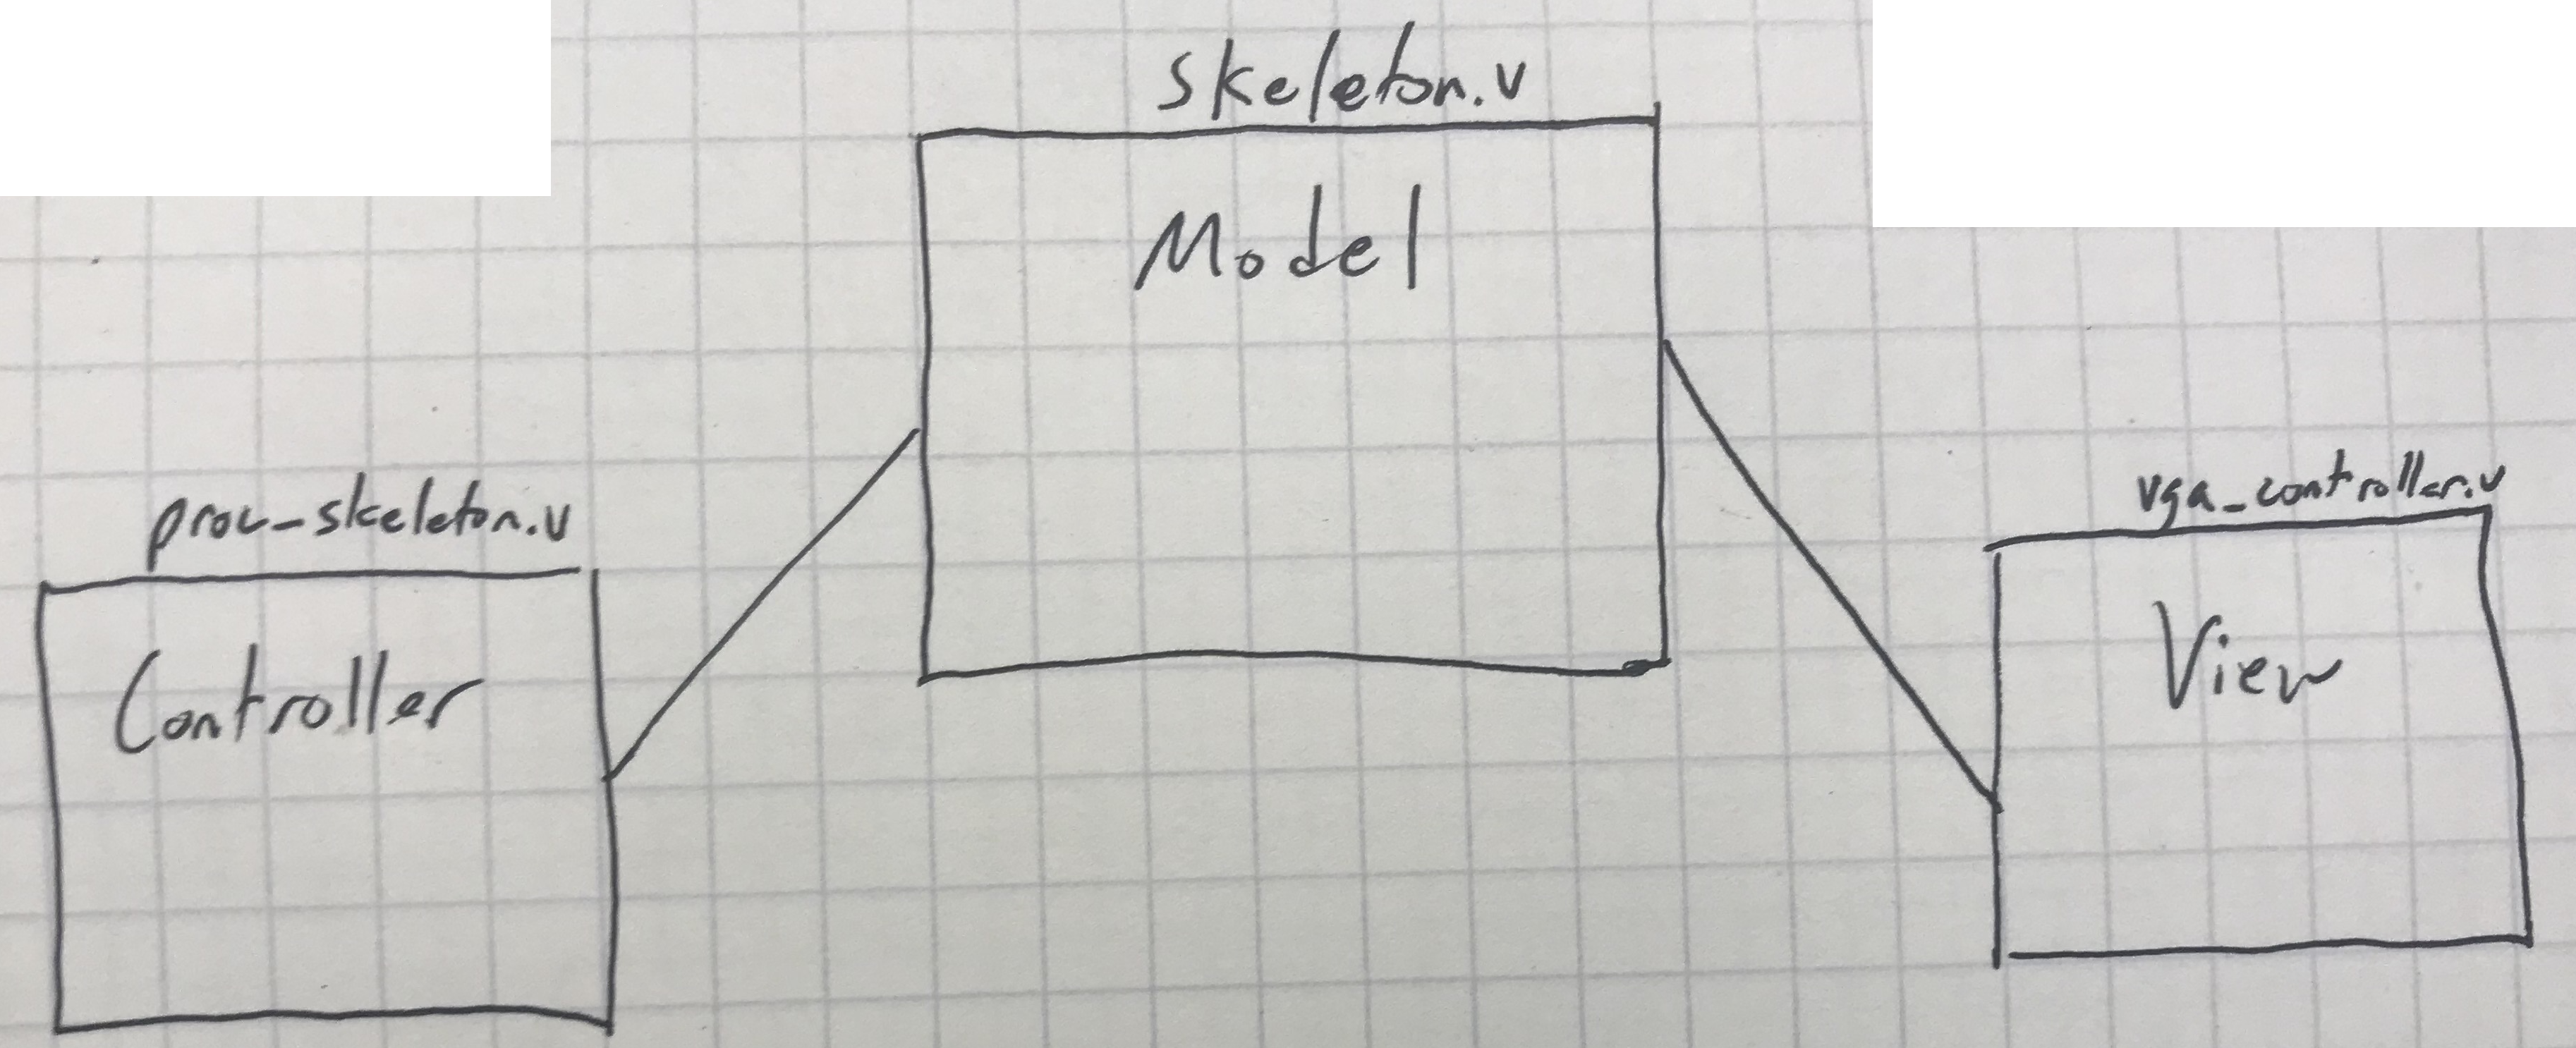
\includegraphics[scale=.05]{MVC}
	\end{center}\par
	The main thing we wanted to ensure for this project was that we kept an MVC model between our processor and the VGA. To do this, we created that concept of Virtual Memory (explained extensively in the Processor Changes section) to allow game element values to be edited by the processor and read by the VGA. Having this in place allowed the VGA to be constantly updated with the processors changing data, but the processor didn't have to sync up with the VGA to make this happen. \par
	A good deal of the visual aids that we played around with made more sense in the VGA controller because they were things that didn't concern the processor. For example, the death sequence we made is several mif files (images of a dying pacman) being cycled through on a counter within the VGA controller. The processor changes the model to indicate that pacman has died, which initiates the VGA controller to start the sequence, but once that happens the processor no longer cares how that command is carried out. \par
	
\section{Input and Output}
	\begin{center}
		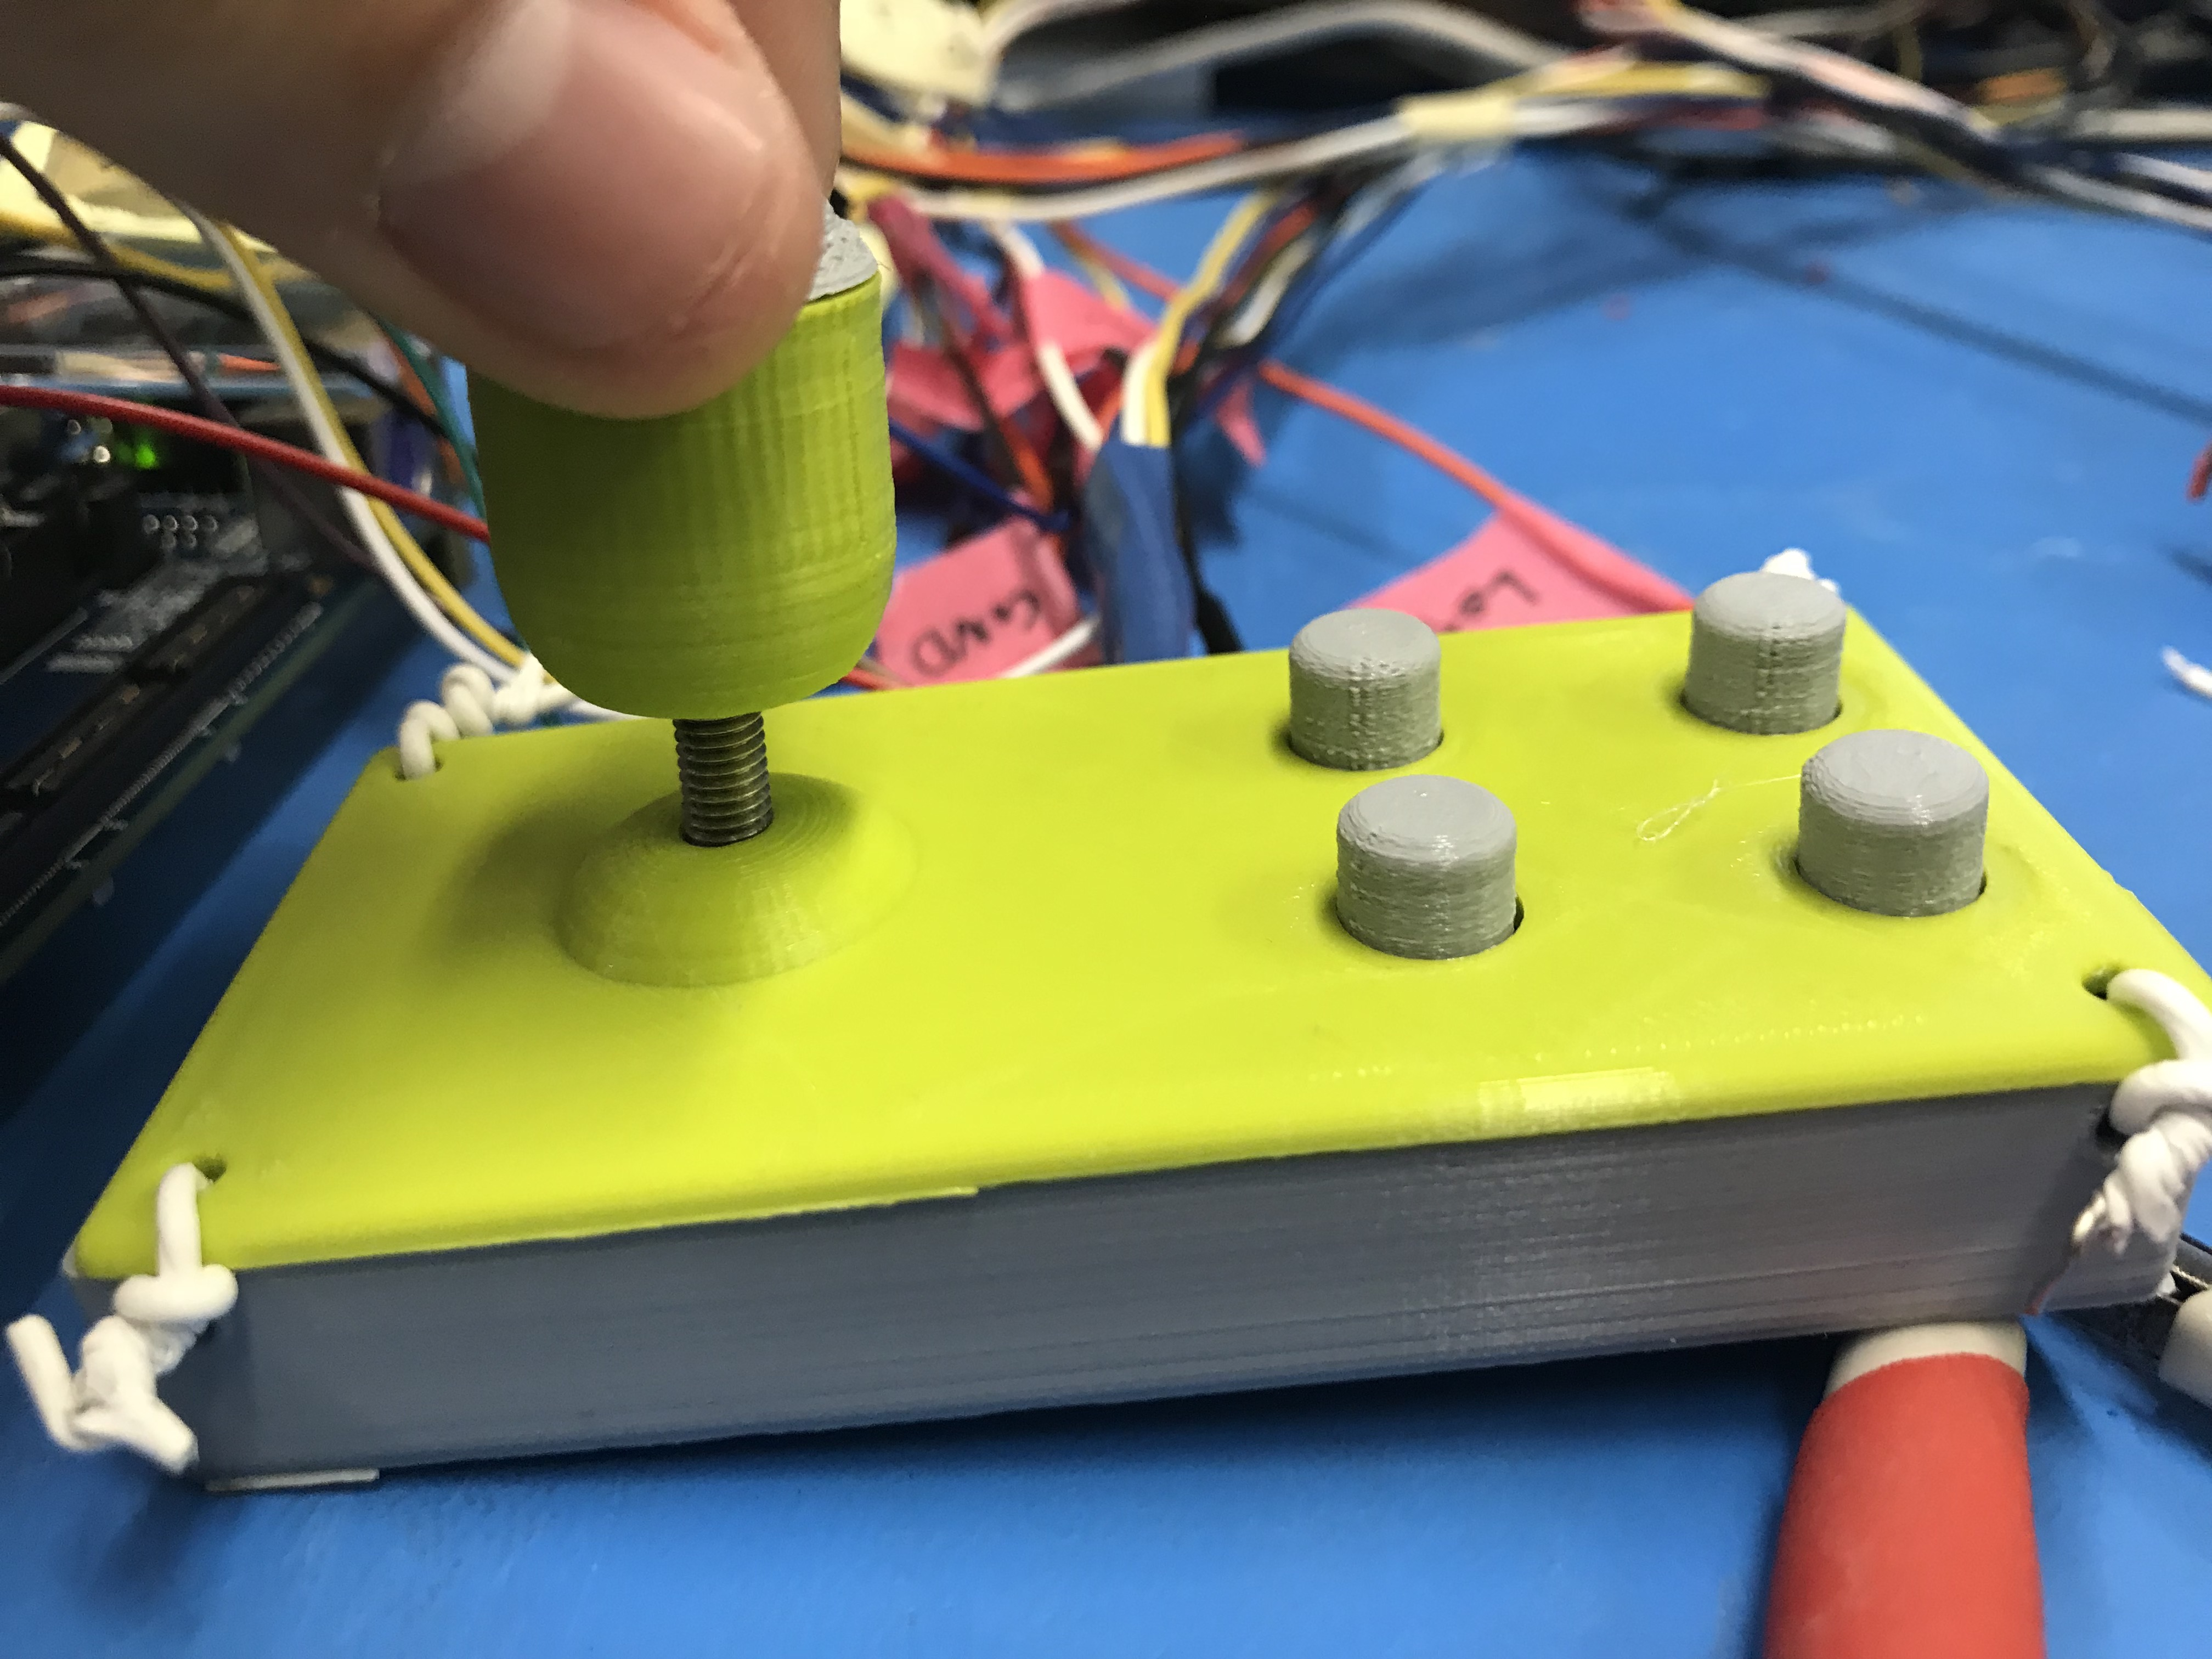
\includegraphics[scale=.07]{controller_closeup}
	\end{center}\par
	The major input to the game are the custom controllers made for the game to react to player input. Throughout testing and even as of now, the switches were really integral as they are a more reliable source of input to the game. The custom controllers have 8 signal inputs, four of which are the cardinal directions for the joystick and the rest of which are four buttons for play/pause/select functionality. If the game had more levels to it with a need for more complex input, we could have taken advantage of all of the inputs that the controllers were designed with. Since we have a very basic game, the joystick and one pause/play button is used to control the game. \par
	The custom game controllers are mechanically very simple. The joystick pushes against buttons in the opposite direction to which the joystick is pushed (like a lever of sorts). Because of this simplicity and the compactness of the design, the joystick feels very responsive and functions well for this purpose. The buttons on the right side of the controller are pressed up against button elements directly below them, so they also feel very responsive and easy to activate.\par
	Also, as a minor addition to the controllers, we glued the female pins of the controller together for easy connection with the FPGA external pins. \par
	\begin{center}
		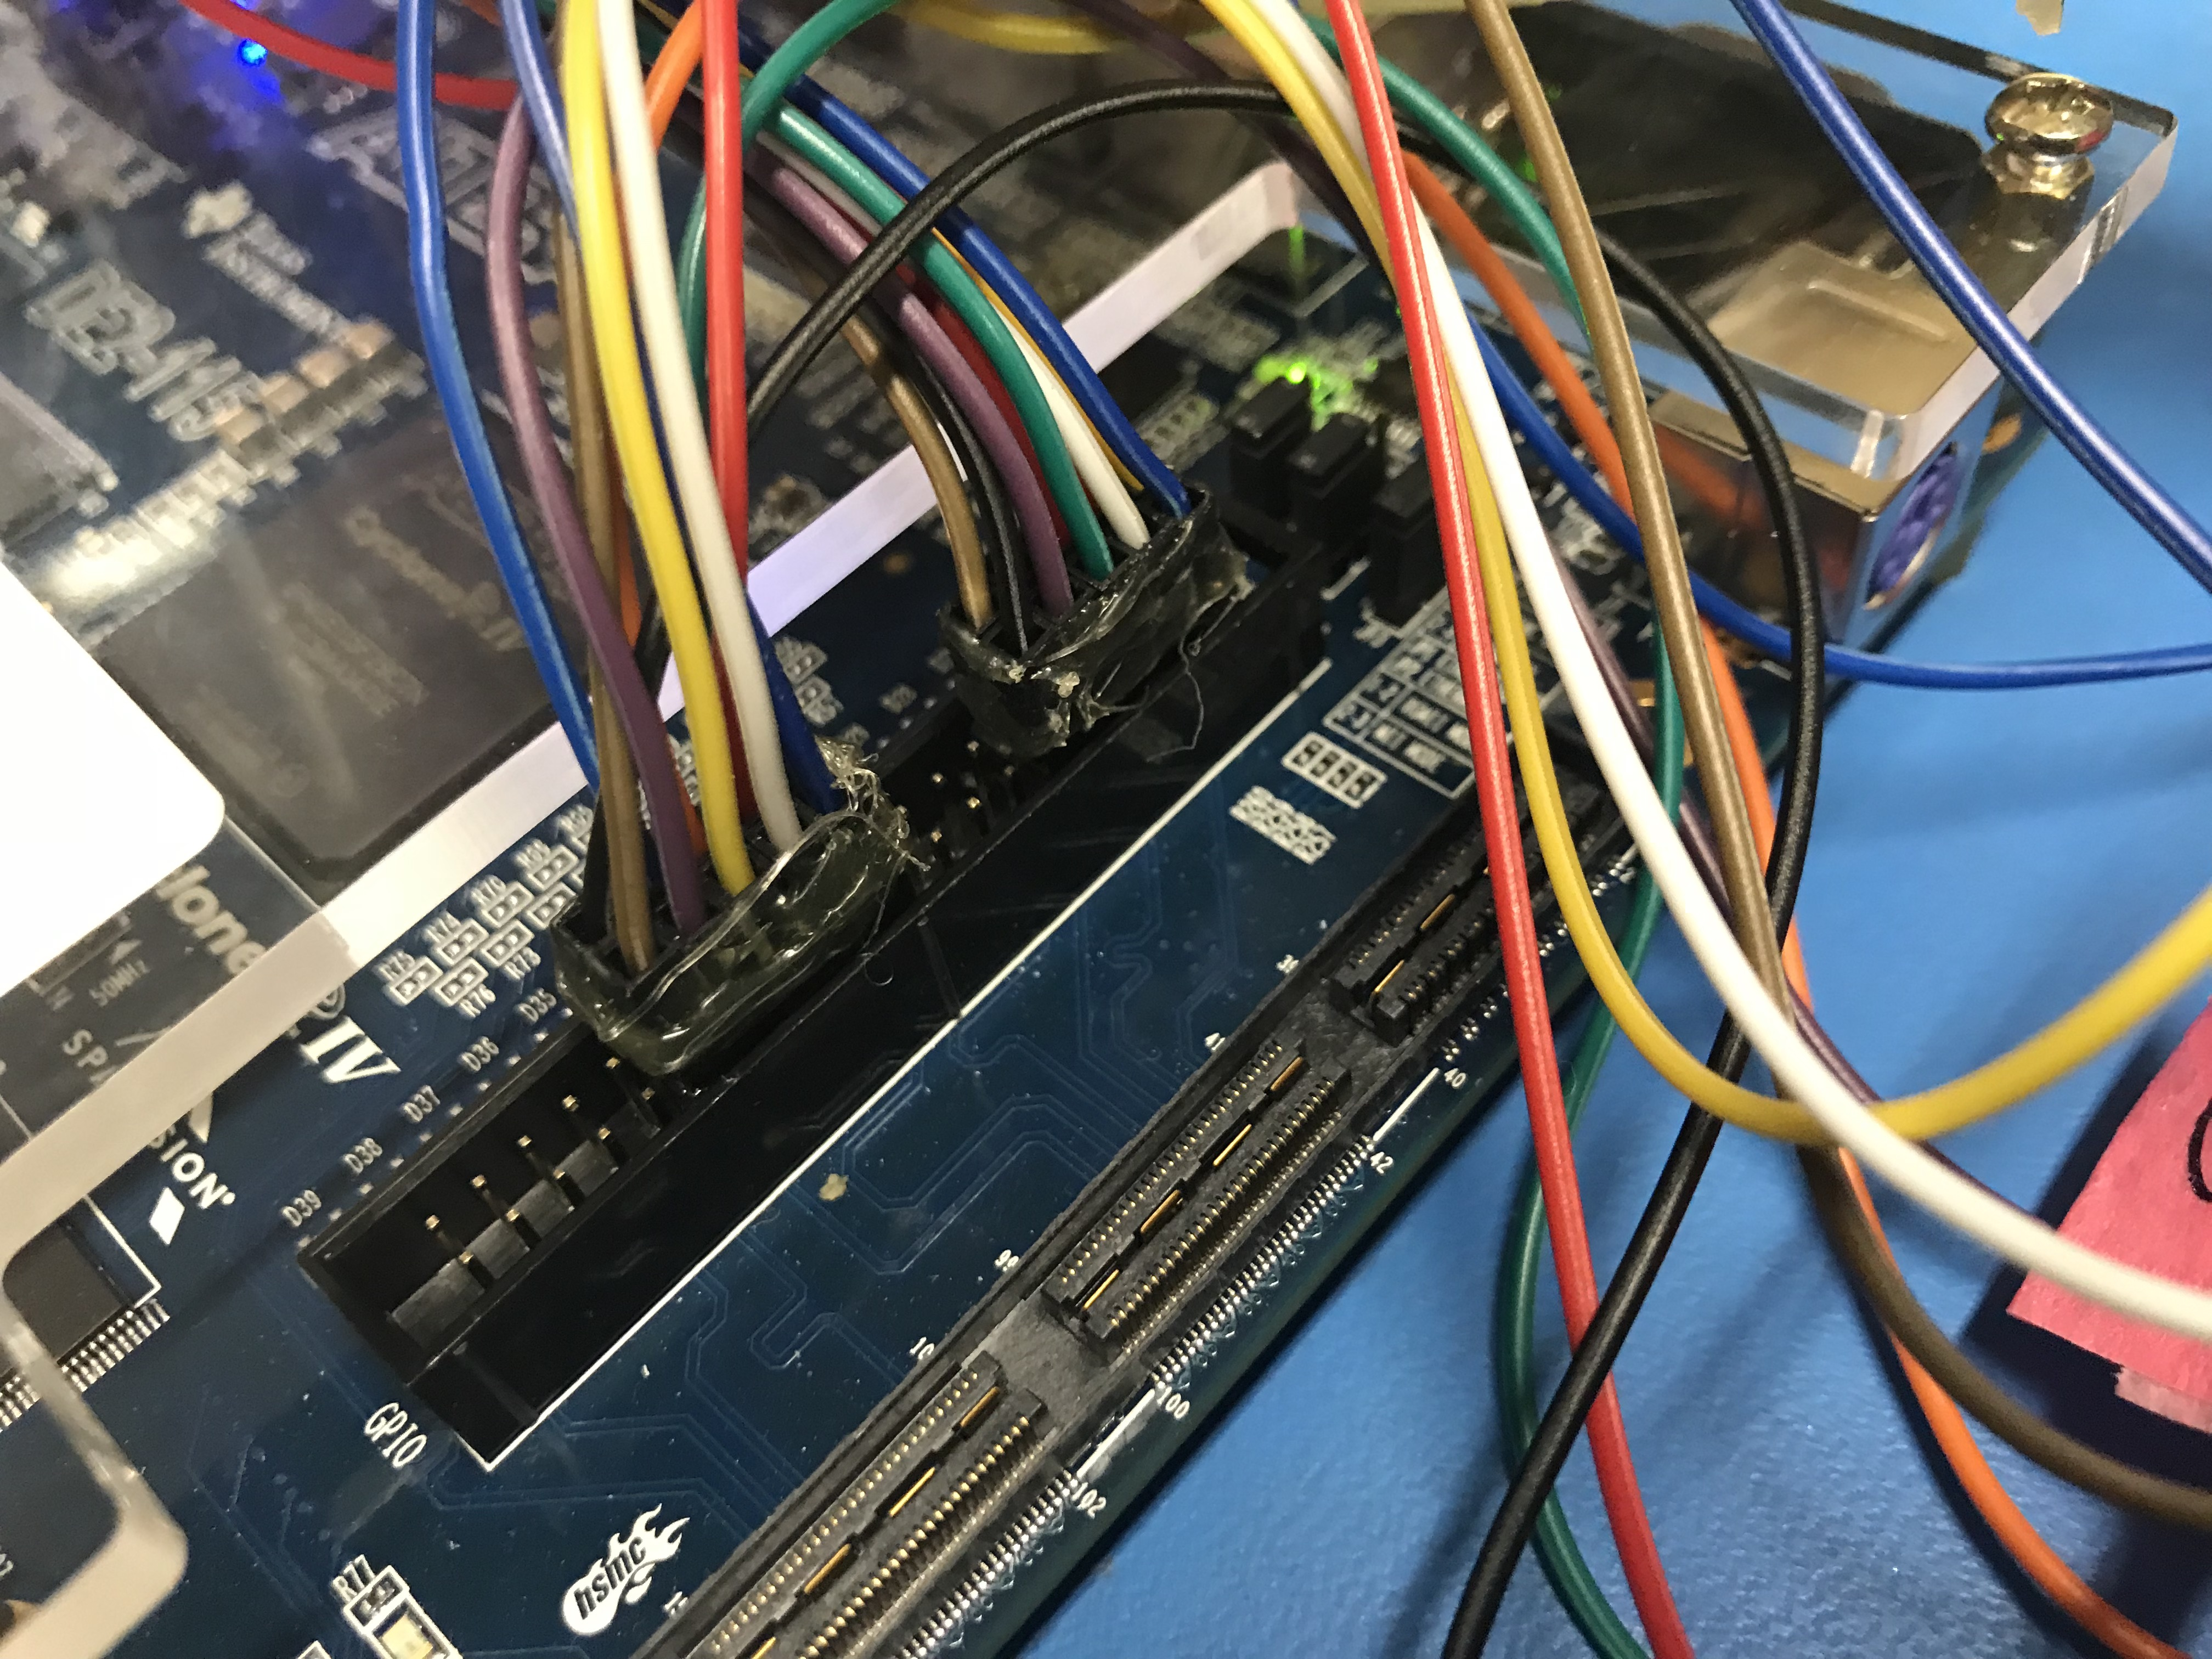
\includegraphics[scale=.07]{fpga_connection}
	\end{center}\par
	The main output for our game was the VGA screen. We essentially refactored the VGA code from labs to show our Pacman interface. There's not much that needs to be said about the VGA output, it was essentially a multiplexing of our game background and the game elements. A cool facet to our design, which is described above, is that we implemented an MVC design scheme where all of the Model game elements (Pacman, Ghosts, etc) were maintained within Virtual Memory outside of the processor so that the View (the VGA) and the Controller (the processor) could access them easily. By keeping this design scheme, we were able to have the view constantly updated without having to make the processor update the View. \par
	\begin{center}
		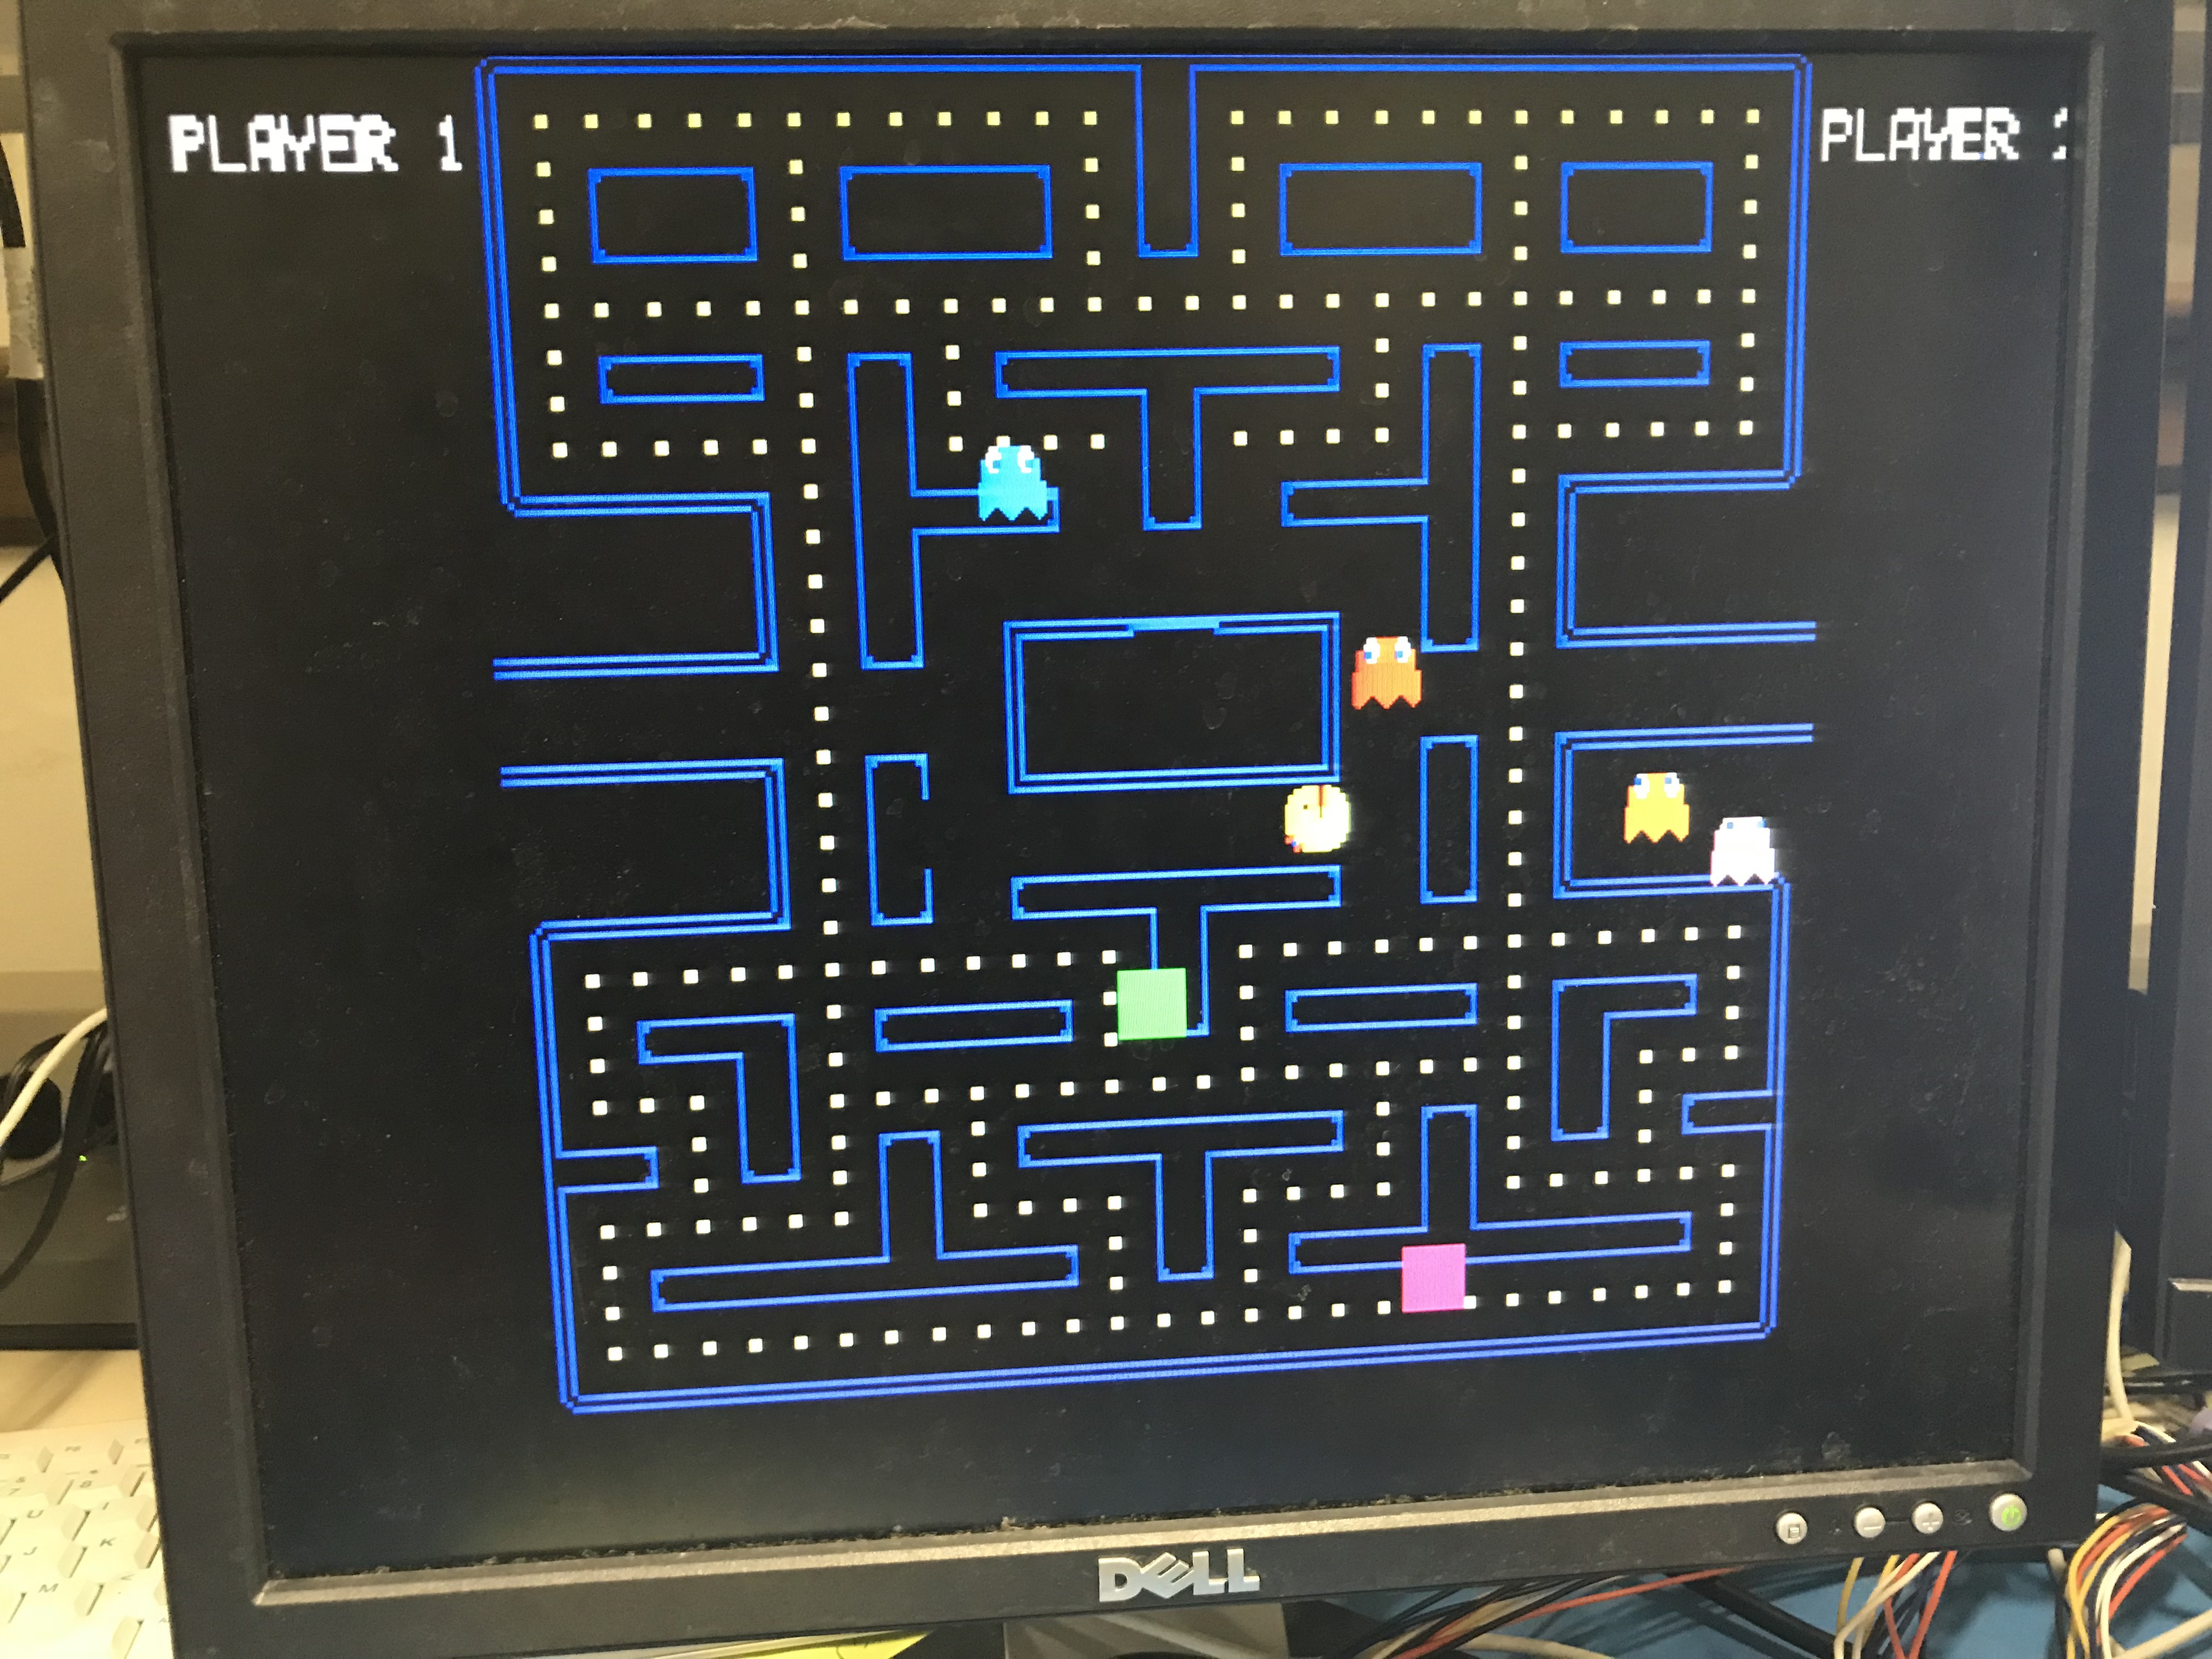
\includegraphics[scale=.07]{vga_screen}
	\end{center}\par
	
\section{Processor Changes}
	We were fortunately able to implement everything for our Pacman game without having to create any new instructions within our processor. The most groundbreaking difference in how we used our processor was the idea of giving it access to Virtual Memory. What this means is that the processor could access its DMEM by accessing memory spots 0 through 4095, however if it had a store-word or load-word instruction for spots about 4095 it would begin to access this Virtual Memory. The Virtual Memory looked like registers in verilog that could be written to by the processor and read by the processor and the View (VGA). We mapped the Virtual Memory Addresses to particular game element values, for example 4100 could be mapped to Player 1's x-location. Fundamentally, we didn't change how the processor functioned, but we essentially made memory that the processor could affect just as easily as the DMEM, but could be read by the View without the processor having to load the data out. Though this takes a good amount of the work away from the processor, we thought this was a pretty ingenious way of keeping all facets of the game up-to-date without having to synchronize the different clocks and stores/loads. \par
	Functionally, it's as if we added Virtual Memory that is easily accessed by both the View and the Controller as in the diagram below. \par
	\begin{center}
		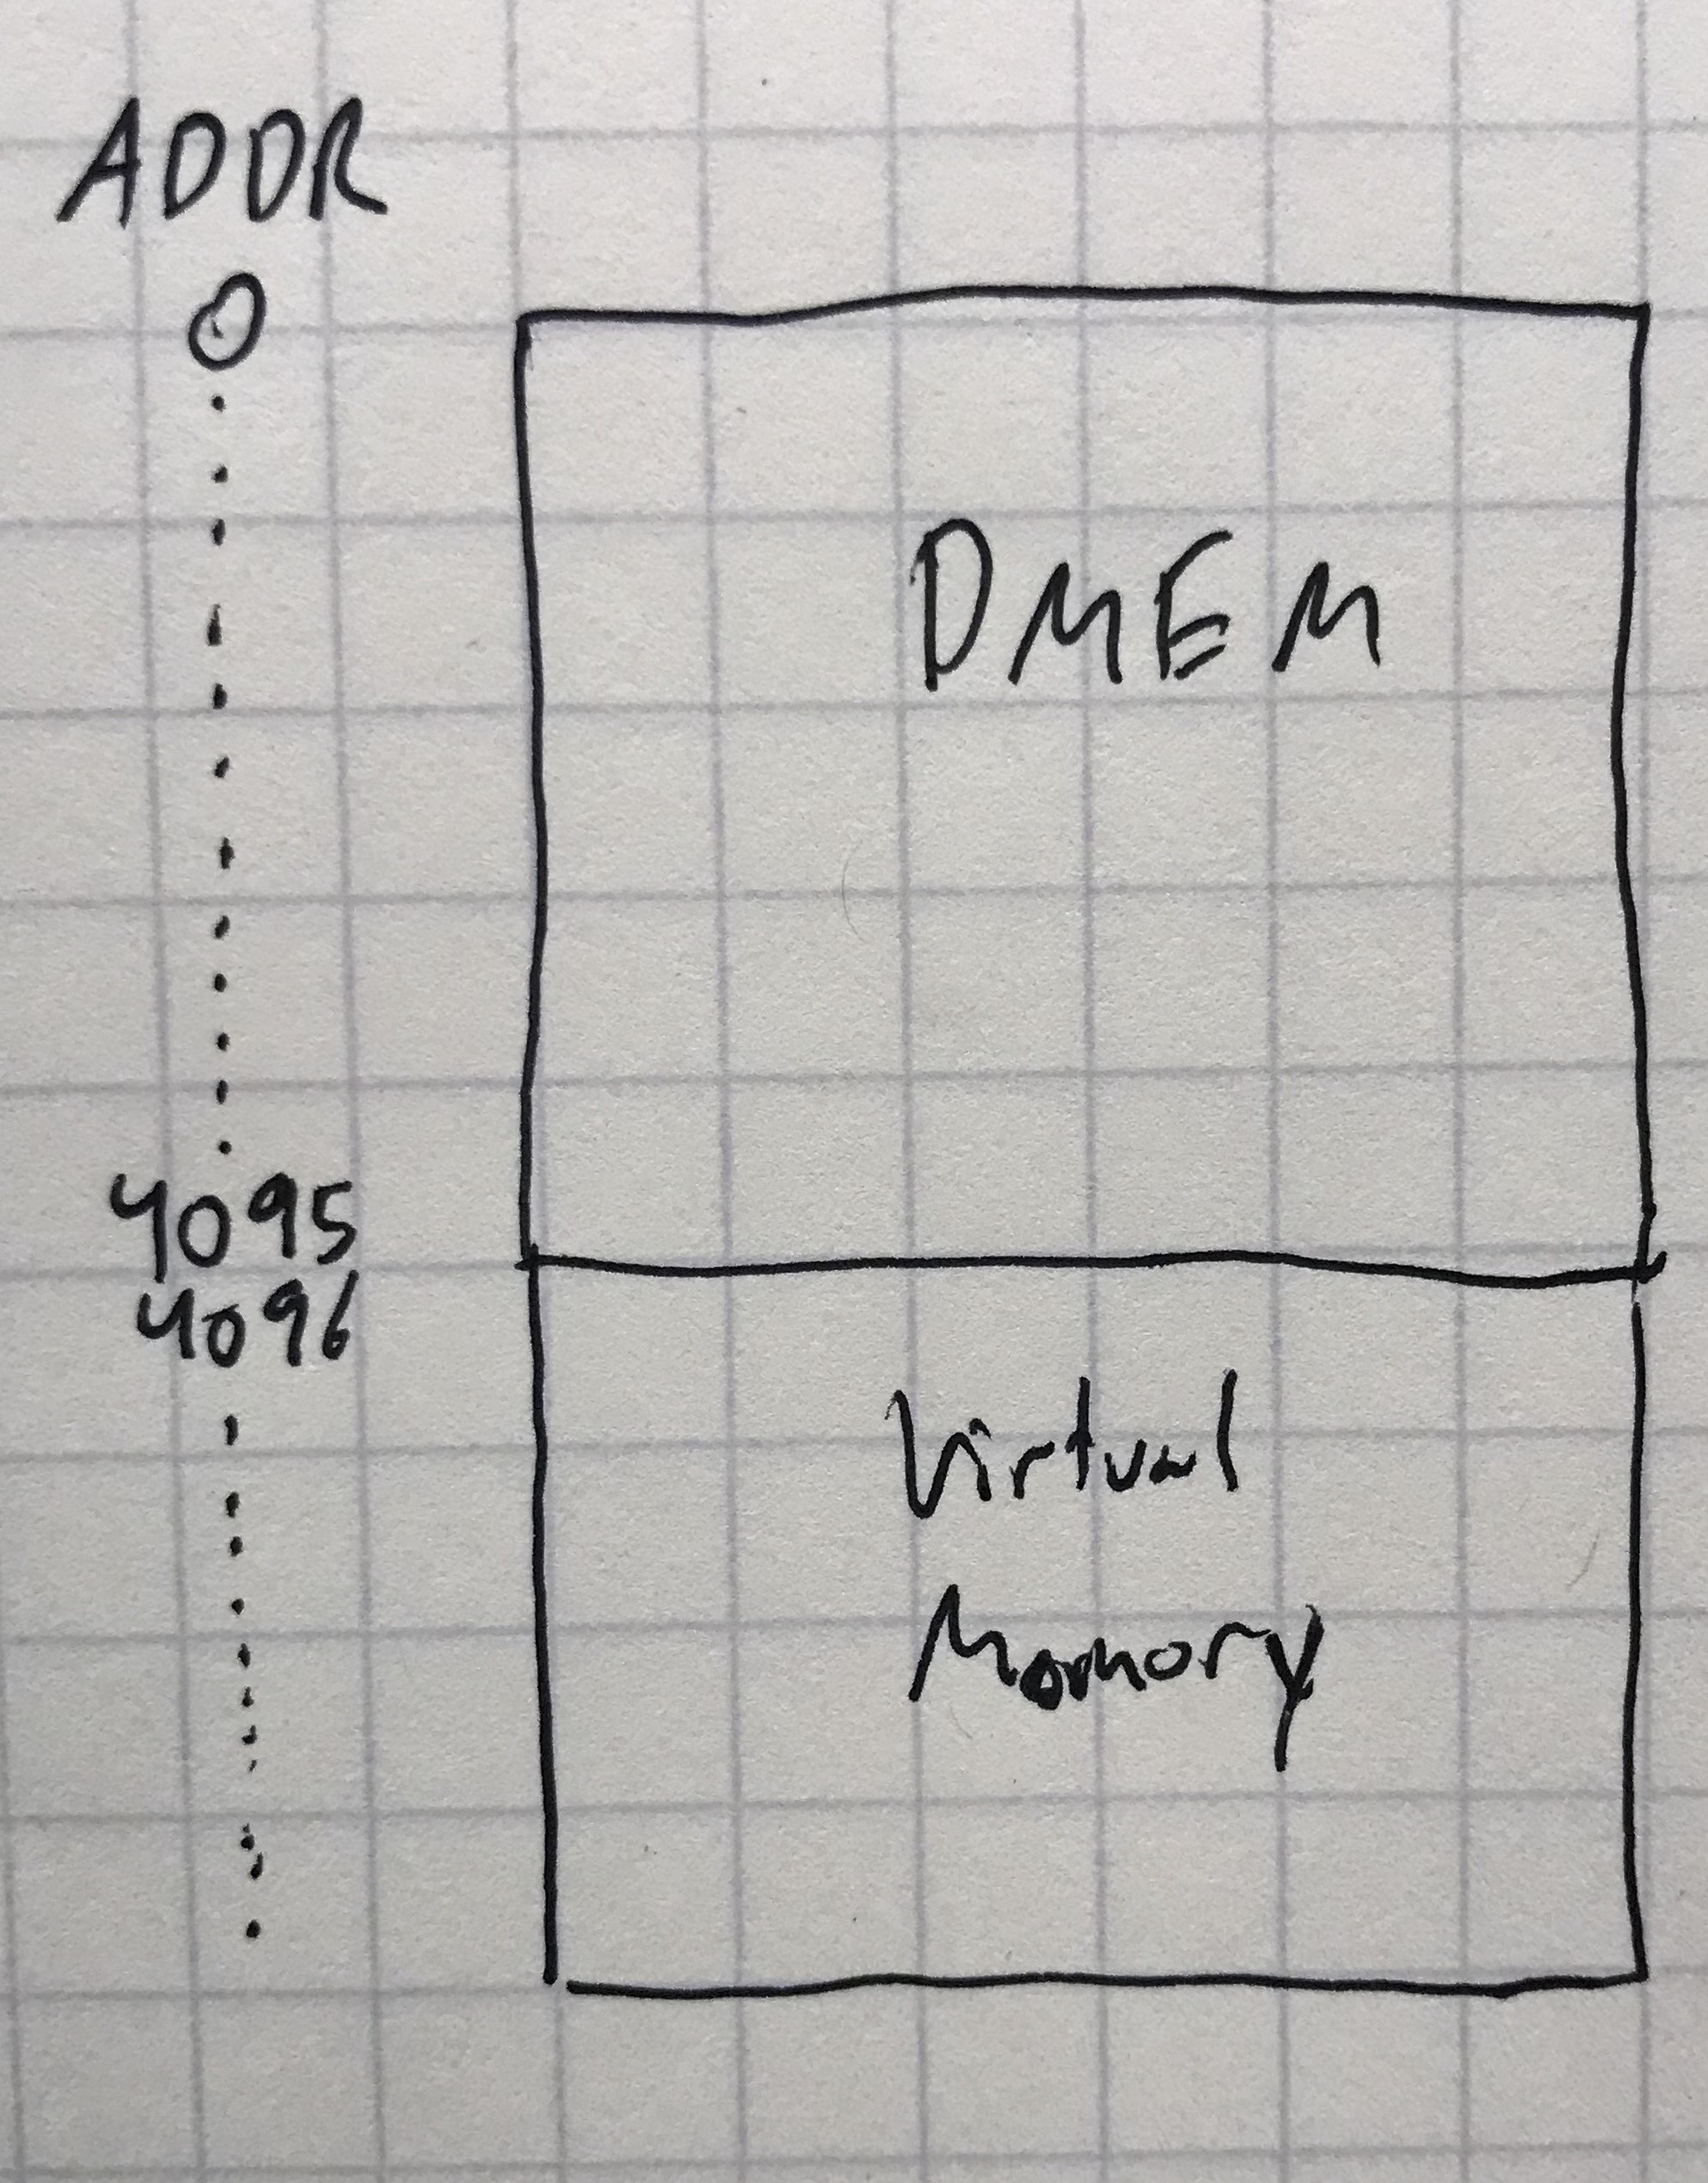
\includegraphics[scale=.05]{virtual_mem}
	\end{center}\par
	The way we actually implemented it was like the diagram below. The storing or loading of words either went directly to the DMEM, or affected other values depending on the particular Virtual Memory Address. \par
	\begin{center}
		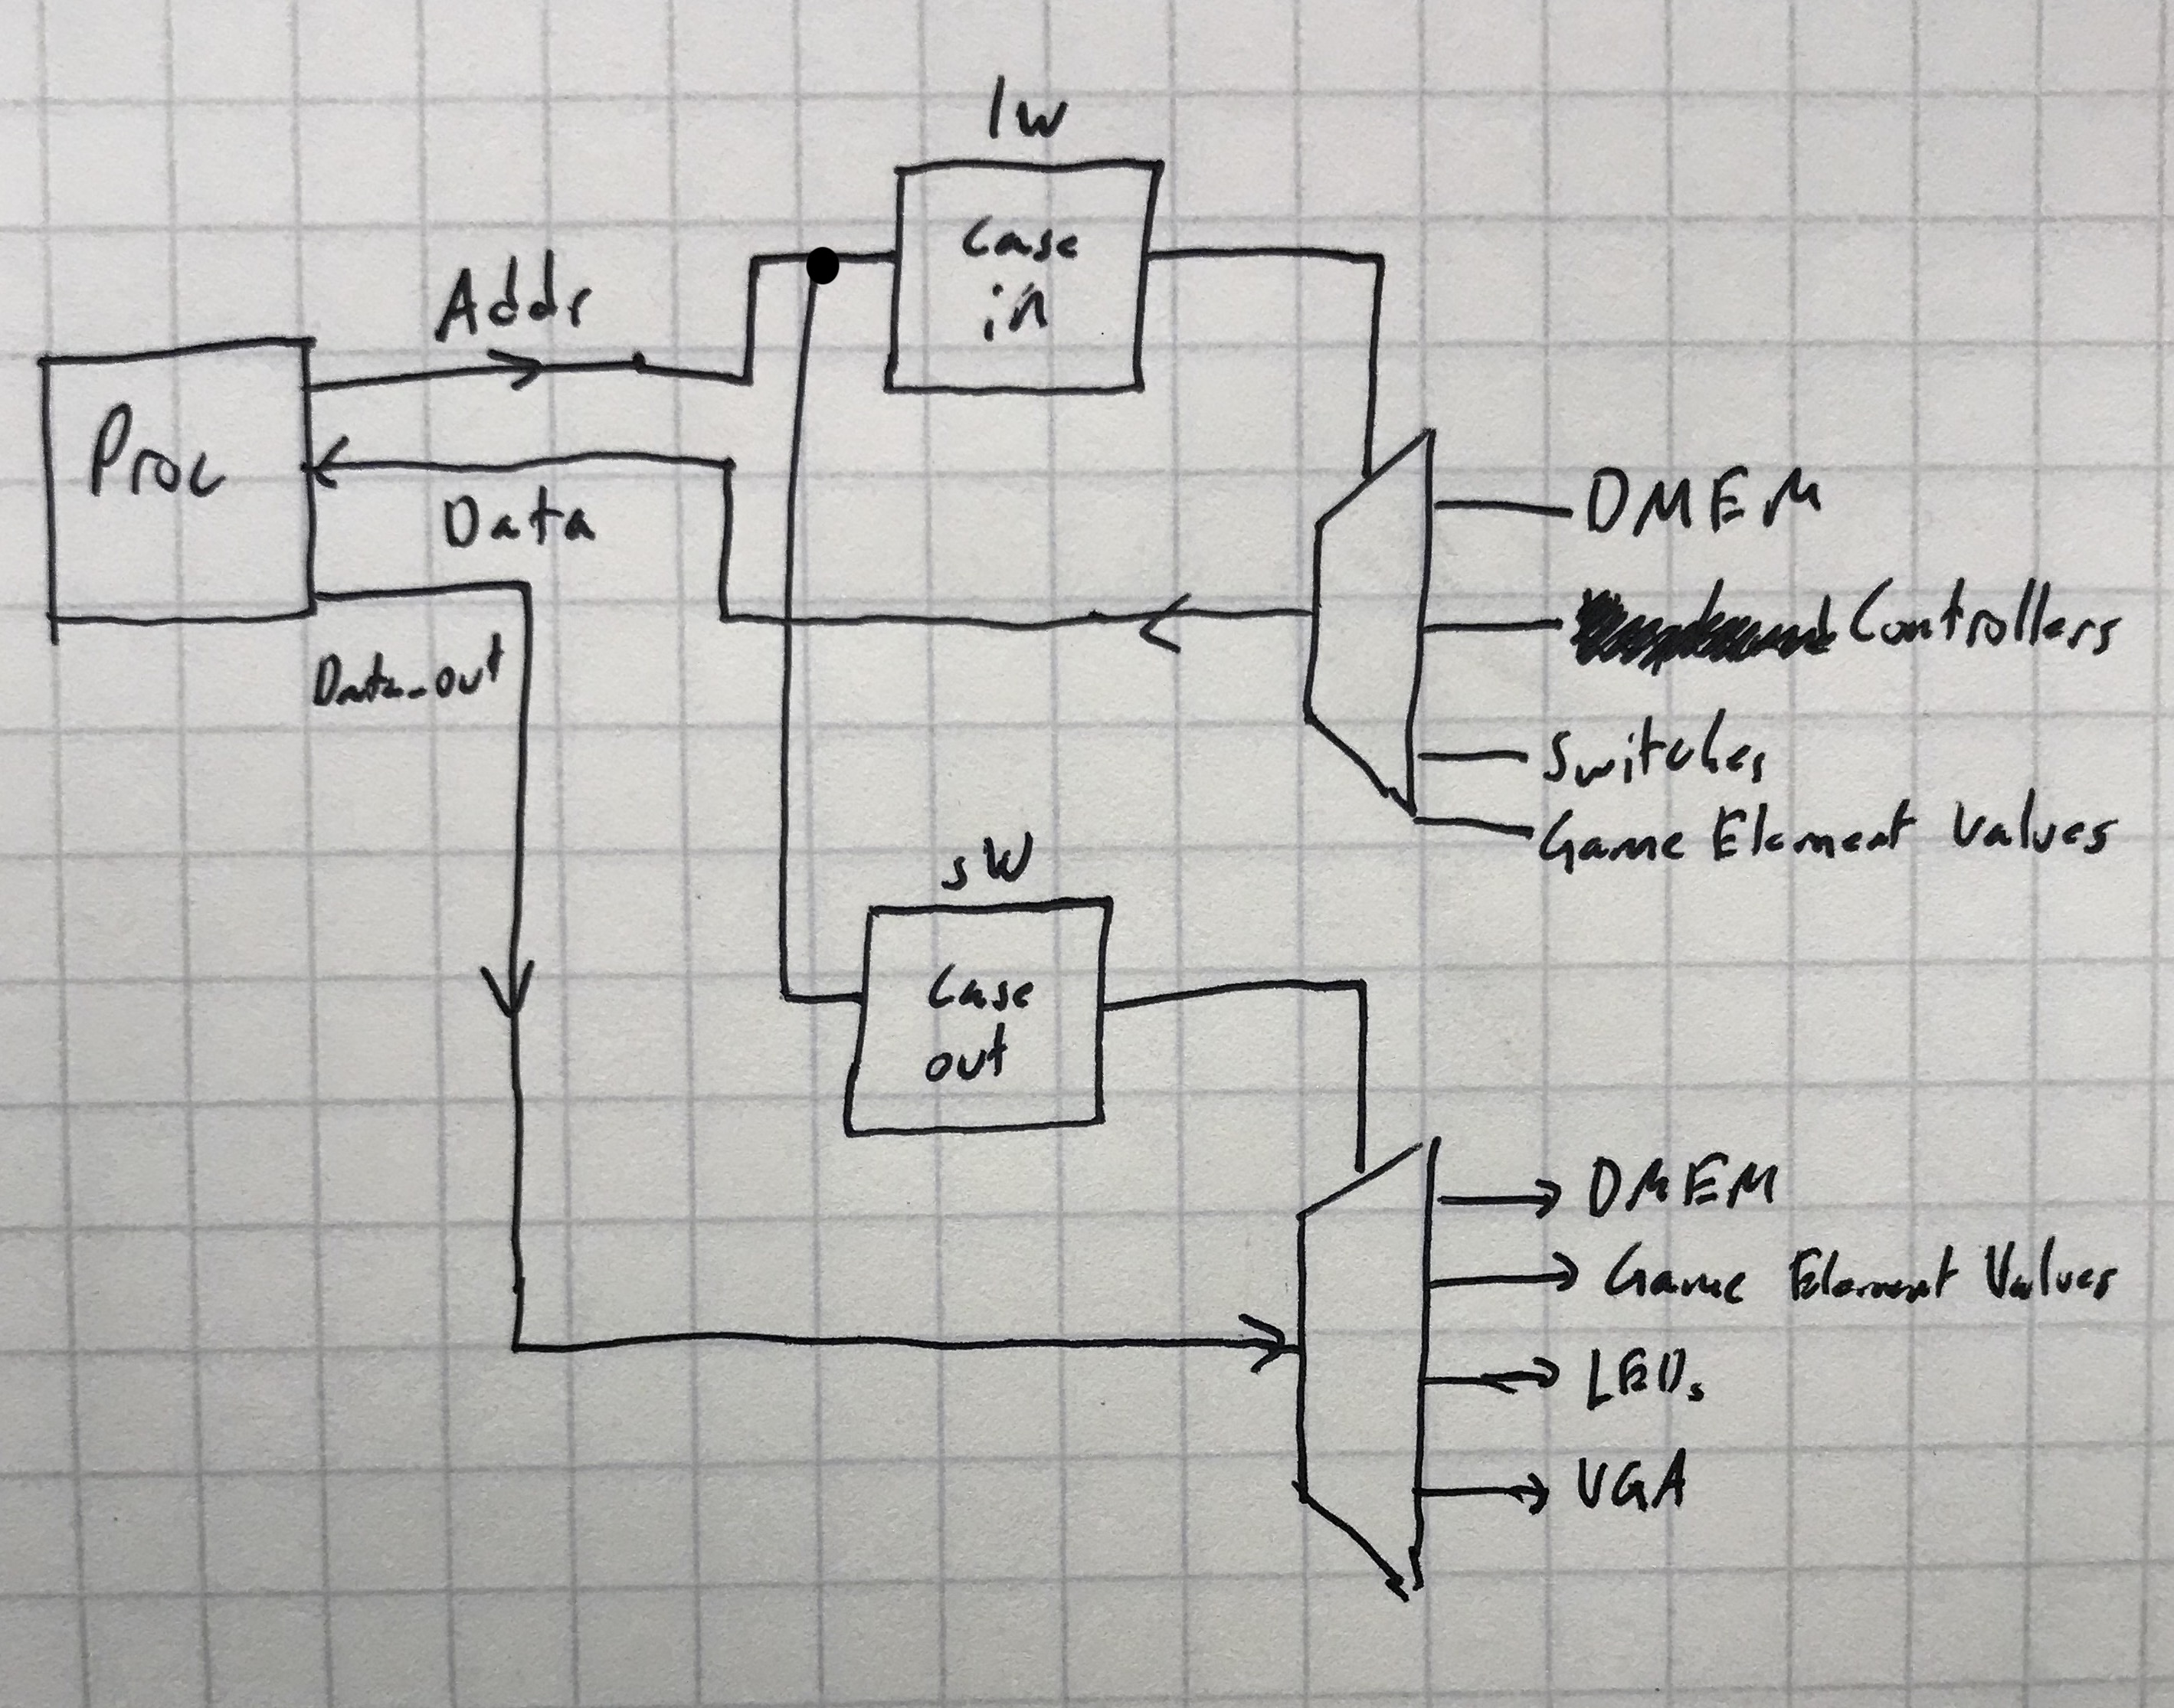
\includegraphics[scale=.1]{VM_diagram}
	\end{center}\par

\section{Challenges}
	The first challenge we faced was to be able to have the VGA constantly updated for the game element locations/states. The reason why this was hard was because if the processor maintained all these values in registers or in DMEM then the VGA wouldn't have constant access to these values. We overcame this by making the MVC model that was described earlier. \par
	The next challenge was also described earlier: the controllers returning all signals high when one button was activated. This was easily remedied by having each button have a pull-down resistor tied to ground as opposed to all of them tied directly to the same ground. \par
	Collision Detection was a pretty large hurdle because there were two main directions that we could take it: we could have collision detection based on the colors of the elements on the screen (if Pacman is about to move on a pixel that is blue, the color of the walls, then detect collision) or  based on hard-coding all of the walls on the screen. We decided it was easier to do the color-detection because hard-coding the wall locations/dimensions would've been a huge pain and still could've not worked well. \par
	Another issue that we ran into was memory space on the FPGA. The memory available to the FPGA for storing mif files and the likes is very low, so we couldn't store very color-intensive pictures on the FPGA to be displayed on the VGA. To get around this problem, we chose pictures with less colors so as to reduce the amount of encoding bits for the mif files. As well, we limited the program to two base background files with minimal colors because those mif files are the largest (307200 entries). \par
	Two main aesthetic changes that we hoped to implement, Pacman's mouth opening/closing and a death sequence for when Pacman is hit by a ghost, couldn't easily be integrated because counters in Verilog don't seem to be functioning properly, thus not muxing the correct mif files in to reflect these dynamic visual effects. We're still working on this feature but we will see if it will end up actually working. \par
	

\section{Circuit Diagrams}
	\begin{center}
		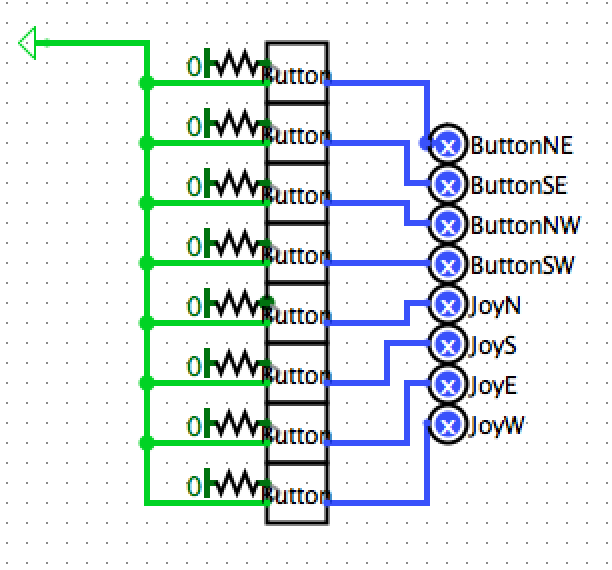
\includegraphics[scale=.8]{controller_diagram}
	\end{center}\par
	
	The only true hardware components that we created were the two game controllers to act as the input for both of the players in the game. Initially, each of the buttons in the controller had been wired to Vcc, GND and a signal wire, but unfortunately when one button is activated in that system, all of the signal wires for the buttons showed high. Clearly this is not useful for a controller with multiple outputs, so the controllers were then changed to reflect an individual pull-down resistor for each of the buttons to ensure that their signals were disconnected. Once that was implemented, the controllers functioned well.\par
	Below is a picture of the actual wiring of the controller. It's hard to see exactly where the wiring is going, but it gives a good idea of how it's laid out and how compact everything is. \par
	\begin{center}
		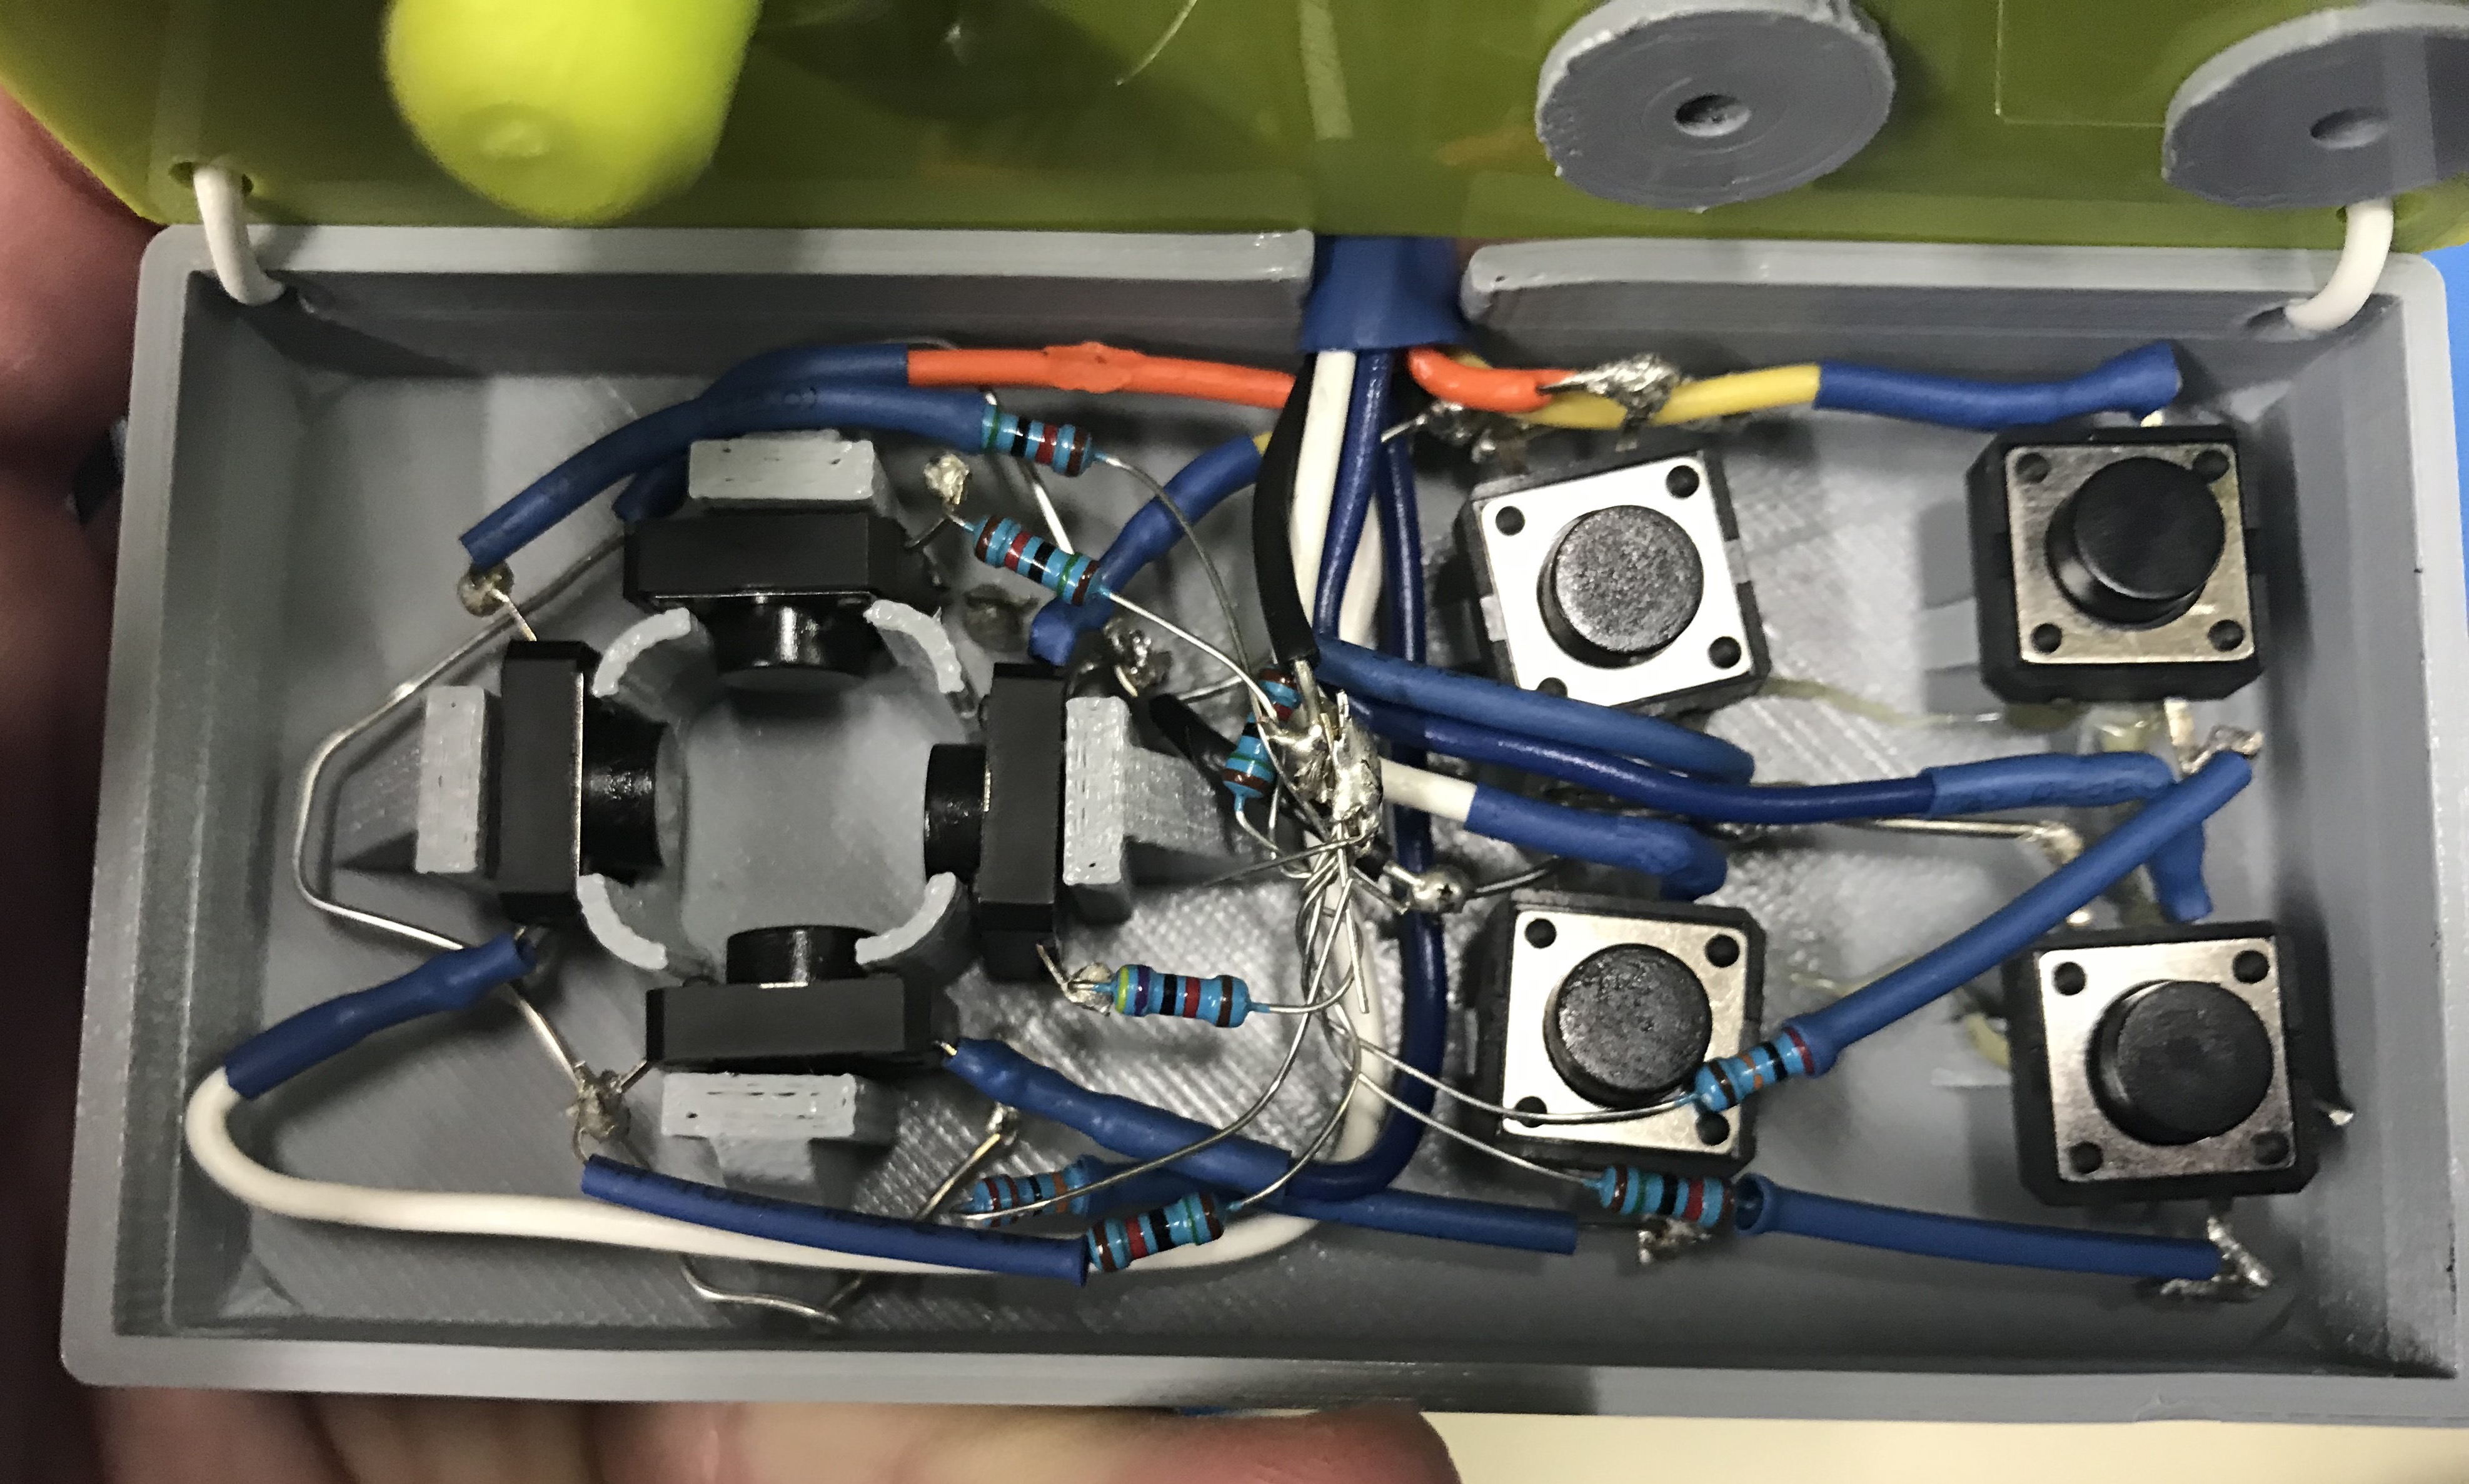
\includegraphics[scale=.08]{controller_internals1}
	\end{center}\par

\section{Testing}
	Our project didn't take much testing, it was mainly making incremental progress until all of it worked. We used the switchea and LEDs on the FPGA excessively to be able to have clear input and output when building our features. Basically, the majority of the issues we ran into were Quartus compile errors, MIF files not being loaded in properly, reading from things in Verilog that shouldn't be read from (i.e. feeding an output into the input of a module) which all didn't really require testing, but they did require us to painstakingly read our code over and over again. We also had to parse through our MIPS code line by line and make sure that we knew what each register was doing. The LEDs we used for testing where mostly to check if a signal was set to high when it should be. The FPGA board was used to print out values (using the 7-segment display) to see if certain values were changing or not (i.e. register values being set, x and y locations being incremented e.t.c). When the custom controllers were done, we had to integrate that as our main input and of course we had to do some testing to ensure they worked properly with all of our input.\par

\section{Assembly Code}

    The assembly code essentially a bunch of sequential checks to see which specific case is occurring. First the code loads in the information stored in our dedicated memory (using a method that George recommended). Then it checks all the information to see what should happen. An example of the logic would be as following: \par
    
    \begin{enumerate}
        \item Load Player input
        \item Check up collision flag
        \item Check if up input is registered
        \item check super speed
        \item if superspeed, up input, and no collision; decrement y by 2
        \item if up input and no collision; decrement y by 1
        \item if no up input or yes collision; do the same for the next direction
    \end{enumerate}
    
    This logic is basically how all the movement works in our MIPS code and is a general skeleton of our code flow. After all these checks occur, we save the updated information back to our dedicated memory for the VGA to read and update the front end with. We also have other miscellaneous features that were included in the MIPS code but they were also complemented by Verilog logic. Movement was the only feature that was done entirely in MIPS code. However, collisions, powerups, and two player (and when we attempted pausing and leaderboard) was done partially in MIPS.
    
 

\section{Assembly Code Flow Chart}

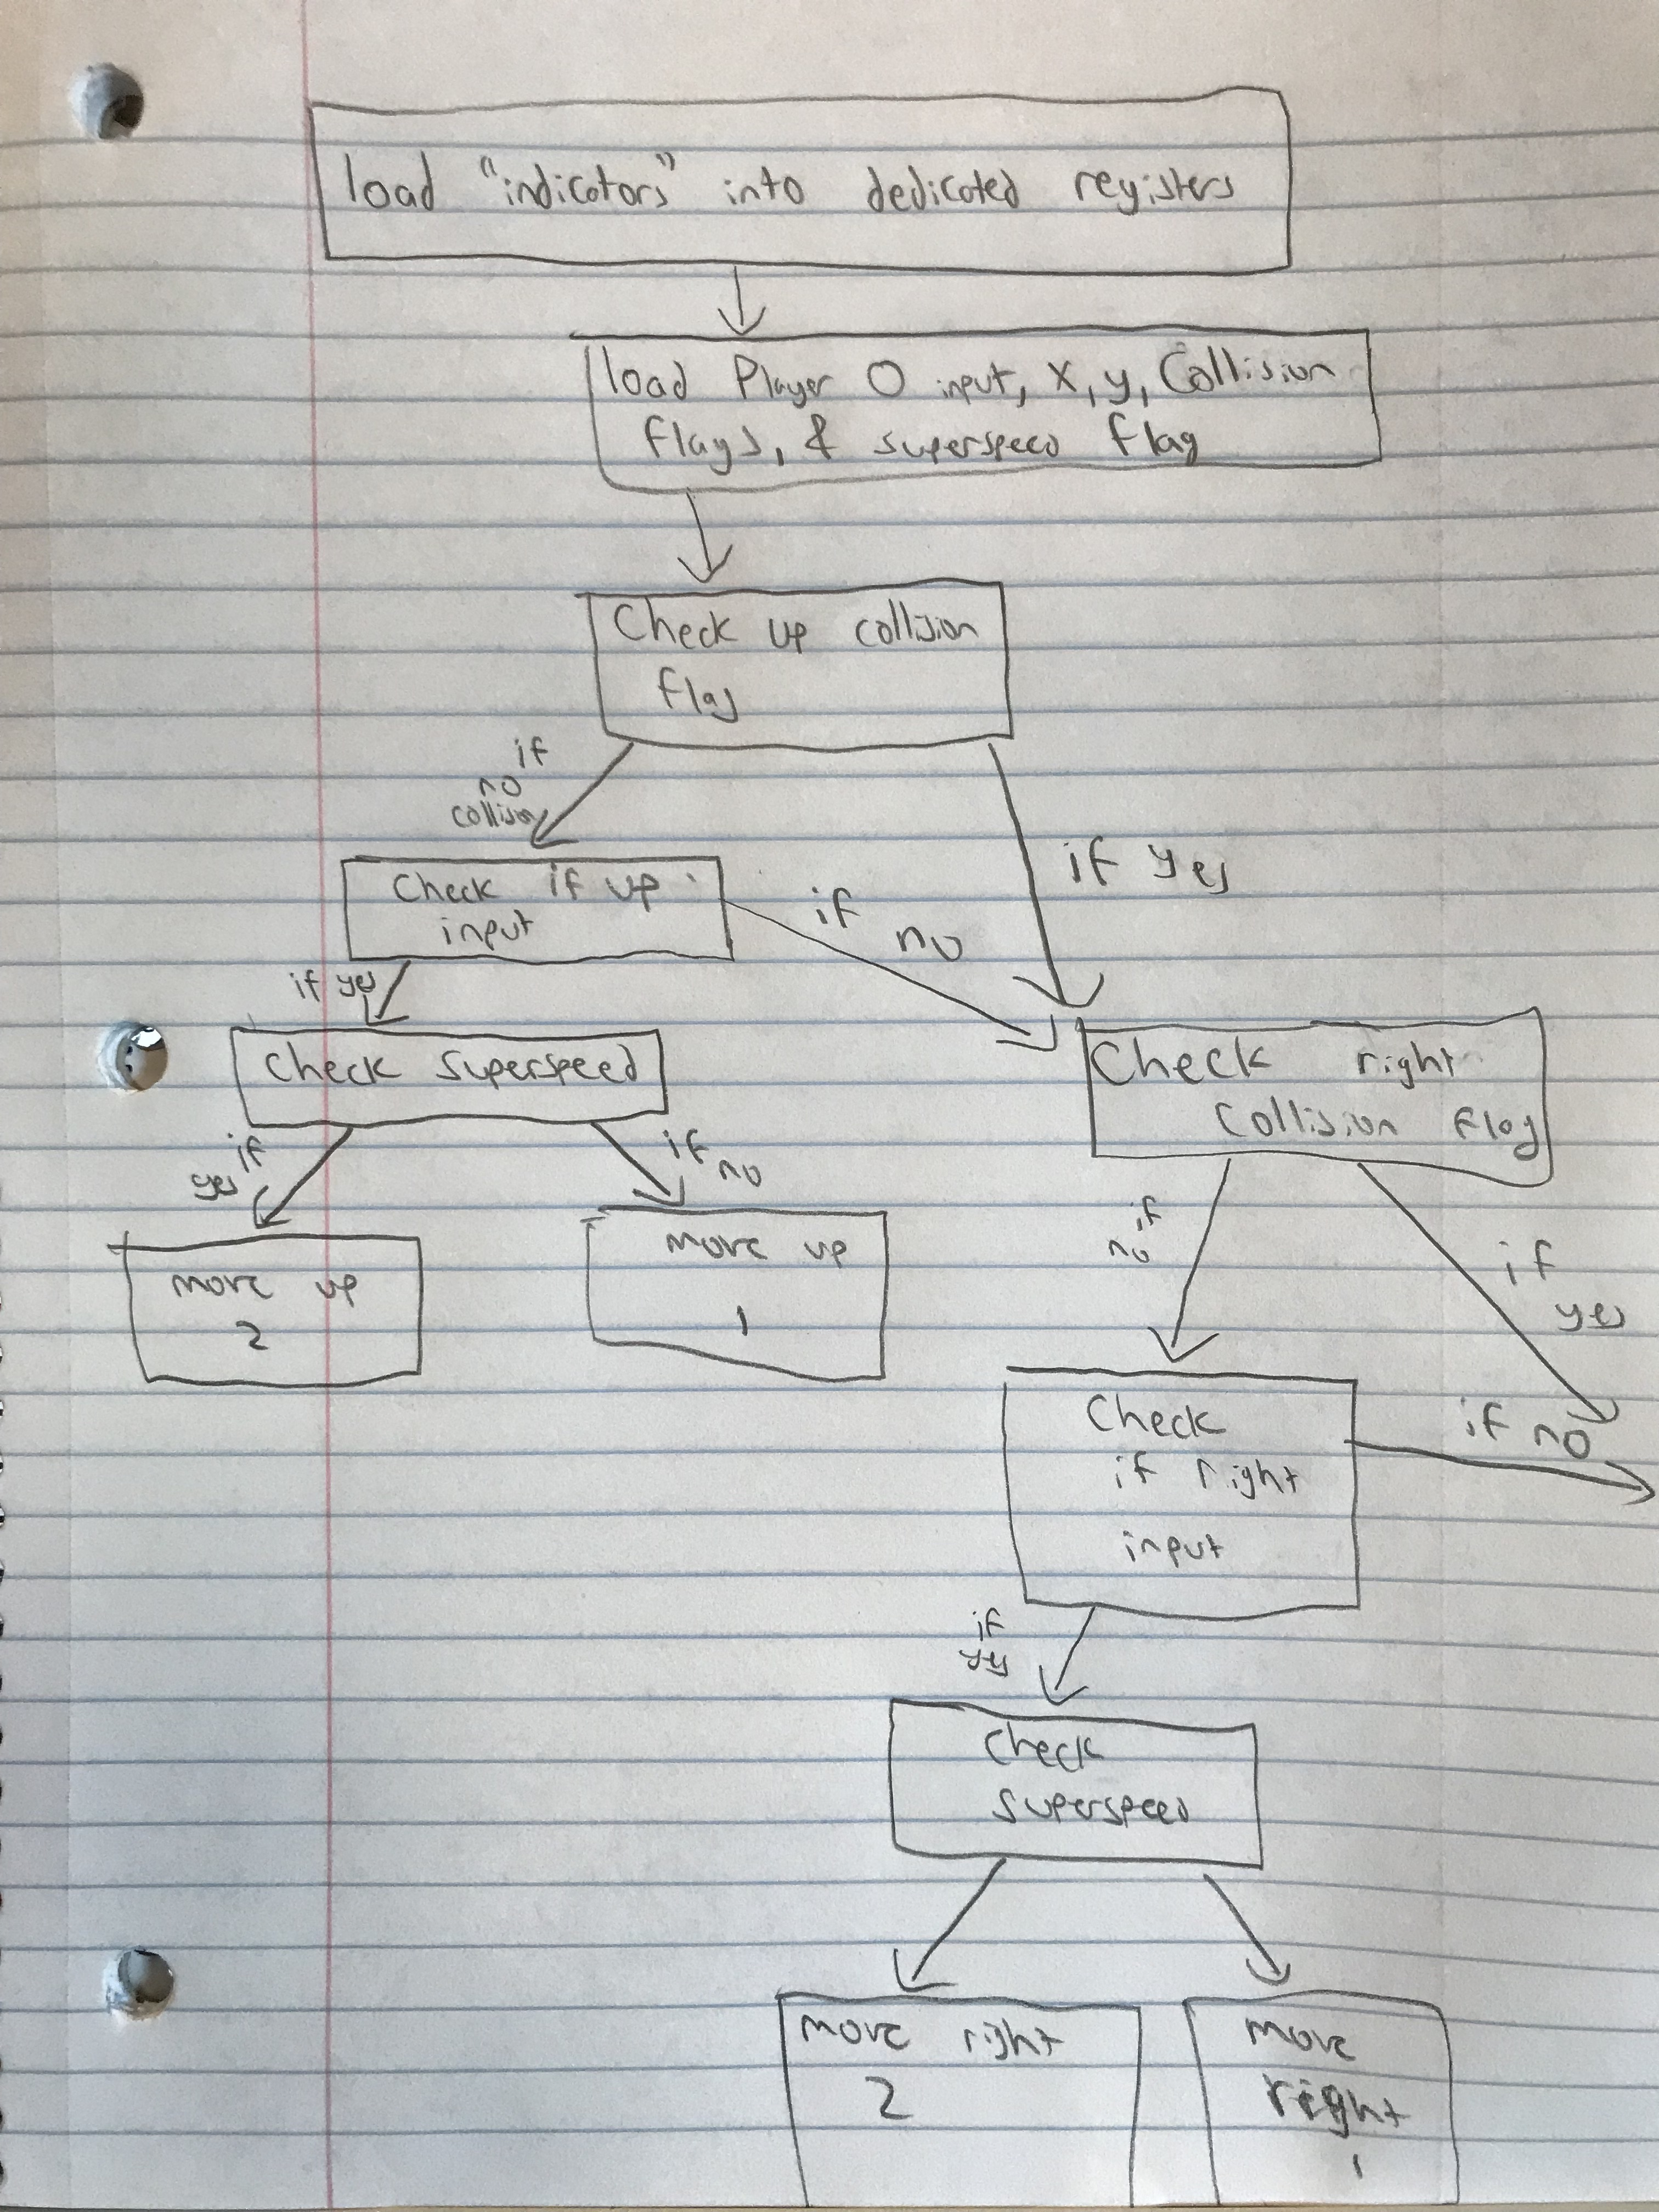
\includegraphics[scale=0.1]{mips_logic.jpg}


\section*{Duke Community Standard}

By submitting this \LaTeX{} document, I affirm that
\begin{enumerate}
    \item I understand that each \texttt{git} commit I create in this repository is a submission
    \item I affirm that each submission complies with the Duke Community Standard and the guidelines set forth for this assignment
    \item I further acknowledge that any content not included in this commit under the version control system cannot be considered as a part of my submission.
    \item Finally, I understand that a submission is considered submitted when it has been pushed to the server.
\end{enumerate}


\end{document}
